\documentclass[tikz,border=14pt]{standalone}
\usepackage{tikz}
\usetikzlibrary{positioning, arrows.meta, calc, backgrounds}

\definecolor{ctrlFill}{RGB}{255,224,189}
\definecolor{ctrlBrd}{RGB}{204,120,30}
\definecolor{compFill}{RGB}{255,252,204}
\definecolor{compBrd}{RGB}{180,160,40}
\definecolor{locFill}{RGB}{210,235,210}
\definecolor{locBrd}{RGB}{90,150,90}
\definecolor{gloFill}{RGB}{210,225,245}
\definecolor{gloBrd}{RGB}{80,110,180}
\definecolor{gmFill}{RGB}{245,210,210}
\definecolor{gmBrd}{RGB}{180,80,80}
\definecolor{keyBg}{RGB}{245,245,245}

\tikzset{
  every node/.style={font=\ttfamily\small},
  B/.style={draw, rounded corners=1pt, inner sep=4pt, align=center, minimum height=0.65cm},
  CTRL/.style={B, fill=ctrlFill, draw=ctrlBrd},
  COMP/.style={B, fill=compFill, draw=compBrd},
  LOC/.style={B,  fill=locFill,  draw=locBrd},
  GLO/.style={B,  fill=gloFill,  draw=gloBrd},
  GM/.style={B,   fill=gmFill,   draw=gmBrd},
  AR/.style={-{Stealth[length=5pt]}, thick, black, shorten >=8pt, shorten <=8pt},
}

\newcommand{\vflow}[2]{\draw[AR] (#1.south) -- (#2.north);}

\begin{document}
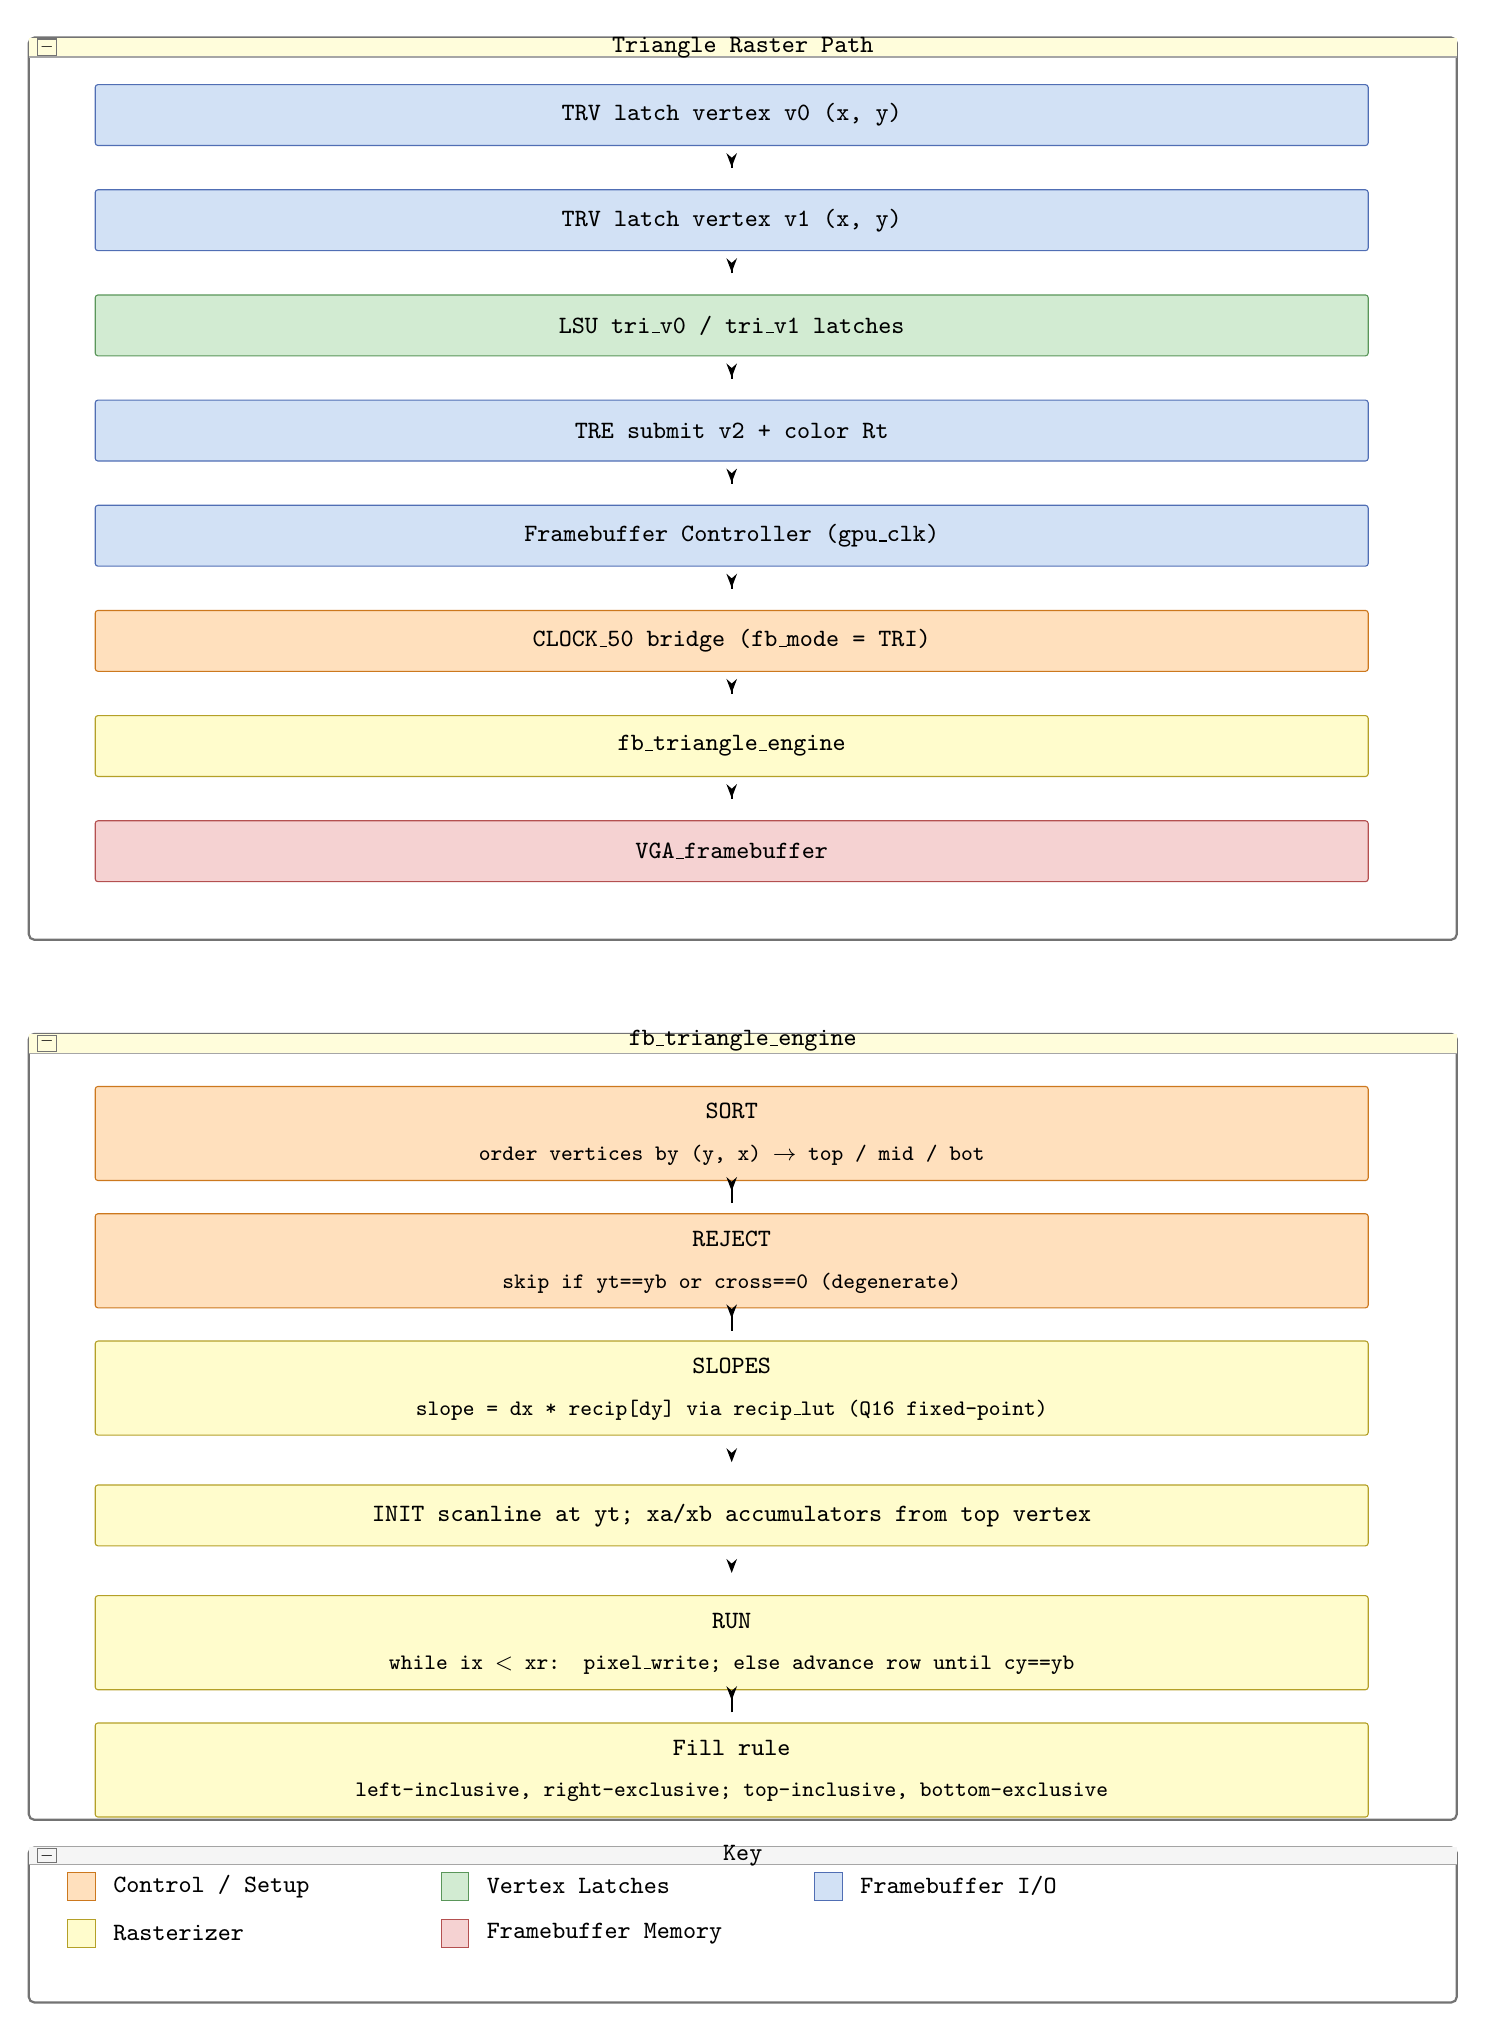
\begin{tikzpicture}[x=1pt, y=1pt, yscale=-1]

\def\W{460pt}
\def\cx{260}

%% ═══════════════════════════════════════════════════════════════════════════
%%  Panel A — end-to-end triangle raster path
%% ═══════════════════════════════════════════════════════════════════════════

\node[GLO, minimum width=\W, minimum height=22pt] (TRV0) at (\cx,16)
  {\textbf{TRV} latch vertex v0 (x, y)};
\node[GLO, minimum width=\W, minimum height=22pt] (TRV1) at (\cx,54)
  {\textbf{TRV} latch vertex v1 (x, y)};
\node[LOC, minimum width=\W, minimum height=22pt] (LAT) at (\cx,92)
  {LSU tri\_v0 / tri\_v1 latches};
\node[GLO, minimum width=\W, minimum height=22pt] (TRE) at (\cx,130)
  {\textbf{TRE} submit v2 + color Rt};
\node[GLO, minimum width=\W, minimum height=22pt] (FBC) at (\cx,168)
  {Framebuffer Controller (gpu\_clk)};
\node[CTRL, minimum width=\W, minimum height=22pt] (BRG) at (\cx,206)
  {CLOCK\_50 bridge (fb\_mode = TRI)};
\node[COMP, minimum width=\W, minimum height=22pt] (ENG) at (\cx,244)
  {\textbf{fb\_triangle\_engine}};
\node[GM, minimum width=\W, minimum height=22pt] (FB) at (\cx,282)
  {VGA\_framebuffer};

\vflow{TRV0}{TRV1}
\vflow{TRV1}{LAT}
\vflow{LAT}{TRE}
\vflow{TRE}{FBC}
\vflow{FBC}{BRG}
\vflow{BRG}{ENG}
\vflow{ENG}{FB}

\begin{scope}[on background layer]
  \draw[black!55,thick,rounded corners=2pt] (6,-12) rectangle (522,314);
  \fill[compFill!70] (6,-12) rectangle (522,-5);
  \draw[black!35] (6,-5)--(522,-5);
\end{scope}
\node[font=\ttfamily\small\bfseries] at (264,-8.5) {Triangle Raster Path};
\draw[black!55] (9,-11.5) rectangle (16,-5.5);
\node[font=\ttfamily\tiny] at (12.5,-8.5) {$-$};

%% ═══════════════════════════════════════════════════════════════════════════
%%  Panel B — fb_triangle_engine FSM
%% ═══════════════════════════════════════════════════════════════════════════

\def\yTop{348}
\def\yB{384}
\node[CTRL, minimum width=\W, minimum height=34pt] (SORT) at (\cx,\yB) {};
\node[font=\ttfamily\small\bfseries] at (\cx,\yB-8) {SORT};
\node[font=\ttfamily\footnotesize] at (\cx,\yB+8)
  {order vertices by (y, x) $\rightarrow$ top / mid / bot};

\node[CTRL, minimum width=\W, minimum height=34pt] (REJ) at (\cx,\yB+46) {};
\node[font=\ttfamily\small\bfseries] at (\cx,\yB+38) {REJECT};
\node[font=\ttfamily\footnotesize] at (\cx,\yB+54)
  {skip if yt==yb or cross==0 (degenerate)};

\node[COMP, minimum width=\W, minimum height=34pt] (SLP) at (\cx,\yB+92) {};
\node[font=\ttfamily\small\bfseries] at (\cx,\yB+84) {SLOPES};
\node[font=\ttfamily\footnotesize] at (\cx,\yB+100)
  {slope = dx * recip[dy] via recip\_lut (Q16 fixed-point)};

\node[COMP, minimum width=\W, minimum height=22pt] (INIT) at (\cx,\yB+138)
  {INIT scanline at yt; xa/xb accumulators from top vertex};

\node[COMP, minimum width=\W, minimum height=34pt] (RUN) at (\cx,\yB+184) {};
\node[font=\ttfamily\small\bfseries] at (\cx,\yB+176) {RUN};
\node[font=\ttfamily\footnotesize] at (\cx,\yB+192)
  {while ix $<$ xr: pixel\_write; else advance row until cy==yb};

\node[COMP, minimum width=\W, minimum height=34pt] (FILL) at (\cx,\yB+230) {};
\node[font=\ttfamily\small\bfseries] at (\cx,\yB+222) {Fill rule};
\node[font=\ttfamily\footnotesize] at (\cx,\yB+238)
  {left-inclusive, right-exclusive; top-inclusive, bottom-exclusive};

\vflow{SORT}{REJ}
\vflow{REJ}{SLP}
\vflow{SLP}{INIT}
\vflow{INIT}{RUN}
\vflow{RUN}{FILL}

\def\yBot{632}
\begin{scope}[on background layer]
  \draw[black!55,thick,rounded corners=2pt] (6,\yTop) rectangle (522,\yBot);
  \fill[compFill!70] (6,\yTop) rectangle (522,\yTop+7);
  \draw[black!35] (6,\yTop+7)--(522,\yTop+7);
\end{scope}
\node[font=\ttfamily\small\bfseries] at (264,\yTop+2.5) {fb\_triangle\_engine};
\draw[black!55] (9,\yTop+0.5) rectangle (16,\yTop+6.5);
\node[font=\ttfamily\tiny] at (12.5,\yTop+2.5) {$-$};

%% Key
\def\yKeyTop{642}
\def\yKeyBot{698}
\begin{scope}[on background layer]
  \draw[black!55,thick,rounded corners=2pt] (6,\yKeyTop) rectangle (522,\yKeyBot);
  \fill[keyBg] (6,\yKeyTop) rectangle (522,\yKeyTop+6);
  \draw[black!35] (6,\yKeyTop+6)--(522,\yKeyTop+6);
\end{scope}
\node[font=\ttfamily\small] at (264,\yKeyTop+3) {Key};
\draw[black!55] (9,\yKeyTop+0.5) rectangle (16,\yKeyTop+5.5);
\node[font=\ttfamily\tiny] at (12.5,\yKeyTop+3) {$-$};

\fill[ctrlFill](20,\yKeyTop+9) rectangle(30,\yKeyTop+19); \draw[ctrlBrd](20,\yKeyTop+9) rectangle(30,\yKeyTop+19);
\node[anchor=west,font=\ttfamily\small] at (33,\yKeyTop+14) {Control / Setup};
\fill[locFill] (155,\yKeyTop+9) rectangle(165,\yKeyTop+19); \draw[locBrd](155,\yKeyTop+9) rectangle(165,\yKeyTop+19);
\node[anchor=west,font=\ttfamily\small] at (168,\yKeyTop+14) {Vertex Latches};
\fill[gloFill] (290,\yKeyTop+9) rectangle(300,\yKeyTop+19); \draw[gloBrd](290,\yKeyTop+9) rectangle(300,\yKeyTop+19);
\node[anchor=west,font=\ttfamily\small] at (303,\yKeyTop+14) {Framebuffer I/O};
\fill[compFill](20,\yKeyTop+26) rectangle(30,\yKeyTop+36); \draw[compBrd](20,\yKeyTop+26) rectangle(30,\yKeyTop+36);
\node[anchor=west,font=\ttfamily\small] at (33,\yKeyTop+31) {Rasterizer};
\fill[gmFill]  (155,\yKeyTop+26) rectangle(165,\yKeyTop+36); \draw[gmBrd](155,\yKeyTop+26) rectangle(165,\yKeyTop+36);
\node[anchor=west,font=\ttfamily\small] at (168,\yKeyTop+31) {Framebuffer Memory};

\end{tikzpicture}
\end{document}
